%%%%%%%%%% Beamerの初期設定 %%%%%%%%%%%
% beamerを使用する初期設定
\documentclass[aspectratio=169, dvipdfmx, 12pt]{beamer}

% 使用するパッケージ
\usepackage{here, amsmath, latexsym, amssymb, bm, ascmac, mathtools, multicol, tcolorbox, subfig}
\usepackage{braket}
%デザインの選択 (省略可)
\usetheme{Boadilla}
%%%%%%%%%%%%%%%%%%%%%%%%%%%%%%%%%%%%%

%\numberwithin{equation}{section}
%%%%%%%%%% Beamerの基本的なコード %%%%%%%%%%
% 属性
\title{項目反応理論を用いた受験者およびテストの評価}
\author[西郷虎太郎]{熊本大学大学院自然科学教育部博士前期課程\\機械数理工学専攻数理工学教育プログラム \\ 210D8551\ 西郷 虎太郎}
\date{}
% スライドの始まり
\begin{document}

% タイトルページ
\frame{\maketitle}

% 目次ページ
\begin{frame}{目次}
    \tableofcontents
\end{frame}

% 目次の具体例
\section{はじめに}
\begin{frame}{項目反応理論}
  \begin{block}{反応行列$U$}
    受験者$i(i = 1, 2, 3, \cdots, N)$の項目$j(j = 1, 2, 3, \cdots, n)$に対する反応を正答を$1$、誤答を$0$として$u_{ij}$として表す。
    \begin{itemize}
      \item $u_{ij} = 1$(正解のとき)
      \item $u_{ij} = 0$(不正解のとき)
    \end{itemize}
    この$u_{ij}$を$(i,j)$成分にもつ$N\times n$行列$U$ を反応行列$U$という。また、反応行列$U$の第$i$行目を抜き出したベクトル$\boldsymbol{u}_i$を受験者$i$の全項目に対する反応として扱う。
  \end{block}
\end{frame}

\section{準備}
\begin{frame}
    \begin{block}{能力値$\theta$}
      受験者$i$の能力値を$\theta_i$で表す。
    \end{block}
    \begin{block}{識別力$a$}
      推定したい受験者の能力値$\theta$をその項目でどのくらい正確に推定できているのかを表したパラメータである。以下より、項目$j$の識別力を$a_j$で表す。
    \end{block}
    \begin{block}{困難度$b$}
      項目$j$の難しさを表すパラメータであり、$b_j$で表現する。$2$に近いほど能力値$\theta$が高くないと正答できない難しい項目とされる。
    \end{block}
    \begin{block}{偶然率$c$}
      能力値$\theta$に関係なく偶然正答になる確率を表すパラメータである。一般的には、当て推量と呼ばれることもあるが以下では、偶然率という言葉を用いている。項目$j$の偶然率を$c_j$で表す。
    \end{block}

  \end{frame}

%theta_iをつけるのかつけないのか
\begin{frame}
\begin{block}{項目特性関数}
  能力値$\theta_i$の受験者$i$が項目$j$に正解する確率は、受験者の能力値$\theta_i$と項目パラメータに依存するため、正解率を$p_j(\theta_i)$で表す。$p_j(\theta_i)$は $0 \leq p_j(\theta_i) \leq 1 $を満たす$\theta$の増加関数であり,その関数形により項目$j$の能力値$\theta_i$に対する特徴をモデル化することが必要となる.
\end{block}
\begin{block}{正規累積モデル}
標準正規分布の累積分布関数を利用した$\Phi(z) = \int_{-\infty}^{z}\frac{1}{\sqrt{2\pi}} \exp(-\frac{z^2}{2}) dz$を利用する。横軸に能力値$\theta$、縦軸に正答率を配した関数$\Phi(f(\theta))$を正規累積モデルといい、以下のように定義する。
\begin{align}
  \displaystyle
  \Phi(f(\theta))  = \int_{-\infty}^{f(\theta)} \frac{1}{\sqrt{2\pi}} \exp(-\frac{z^2}{2}) dz
\end{align}
\end{block}
\end{frame}

\begin{frame}
  \begin{block}{項目特性関数}
    $\theta$の関数$f(\theta)$を
    \begin{align}
      \displaystyle
        f(\theta) = a(\theta - b)
    \end{align}として、項目$j$の項目特性関数を
    \begin{align}
      \displaystyle
      p_j(\theta) = \Phi (a_j(\theta - b_j))
    \end{align}と表すことができる。
  \end{block}
\end{frame}

\begin{frame}
  \begin{block}{ロジスティックモデル}
    正規累積モデルでは、式中に積分を含んでいるので実際の推定の際には計算が複雑になってしまう。そこでロジスティック分布を利用した項目特性関数が提案された。提案されたモデルは以下のようなものである。
    \begin{align}
      \displaystyle
      \int_{-\infty}^{f(\theta)} \frac{1}{\sqrt{2\pi}} \exp(-\frac{z^2}{2})dz \simeq \frac{1}{1 + \exp(-D \times f(\theta))}
    \end{align}この式の右辺をロジスティックモデルという。一般に、$D = 1.7$のとき、左辺と右辺の誤差が$0.01$以下になることが知られているので今後は$D = 1.7$として扱う。$f(\theta)$に使われる式のパラメータの数によって$1$パラメータロジスティックモデルから$4$パラメータロジスティックモデルまで考えられる。
  \end{block}
\end{frame}
\begin{frame}
    \begin{block}{$1$パラメータロジスティックモデル}
    \begin{align}
      \displaystyle p_j(\theta) = \frac{1}{1+\exp(-Da(\theta - b_j))}
    \end{align}
    これを$1$パラメータロジスティックモデルという。
    \begin{itemize}
      \item[]
      \item $a$は全ての項目に共通している値であるため、項目特性関数は項目同士で交わることはない。
      \item 困難度が高くなるほど、グラフは右に移動していく。
    \end{itemize}
  \end{block}
\end{frame}
\begin{frame}
    \begin{figure}[H]
      \centering
      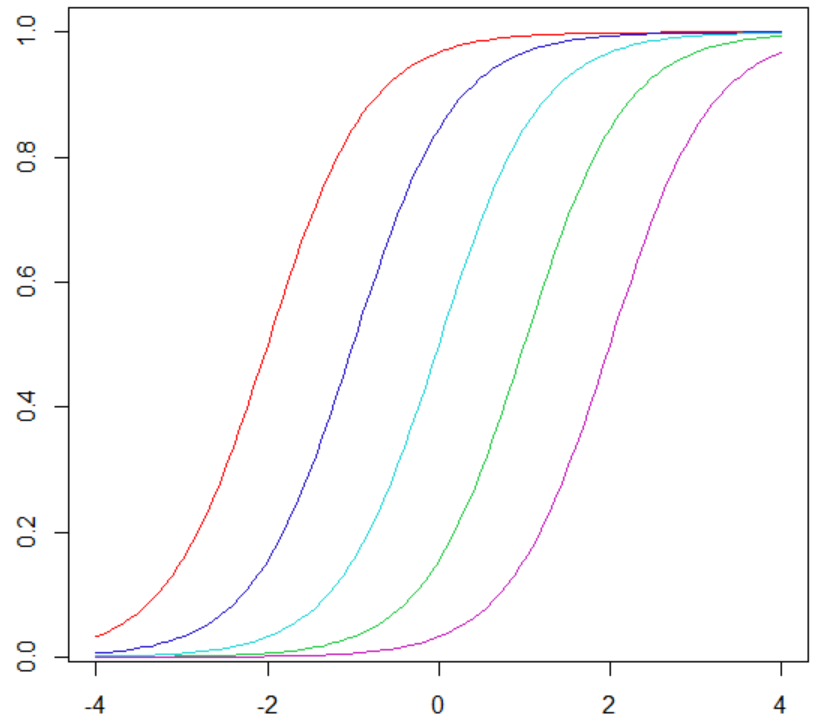
\includegraphics[bb = 500 450 1 1,scale = 0.25]{B.png}
      \vspace{4cm}
      \caption{$a$は$1$で固定、$b$は$-2, -1, 0, 1, 2$}
    \end{figure}
\end{frame}
\begin{frame}
  \begin{block}{$2$母数ロジスティックモデル}
  \begin{align}
    \displaystyle
    p_j(\theta) = \frac{1}{1+\exp(-Da_j(\theta - b_j))}
  \end{align}
  \begin{itemize}
    \item $1$パラメータロジスティックモデルのときとは違い、項目特性関数は項目同士で交わることがある。
    \item 下図のように、$a$の値が大きくなるほどグラフの傾きが大きくなる。つまり、識別力$a$の値が大きくなると、能力値$\theta$の値の少しの変化でも、大きく正答確率が変わることになる。このことから、パラメータ$a$は識別力を表すパラメータを表していることが分かる。
  \end{itemize}
\end{block}
\end{frame}
\begin{frame}
  \begin{figure}[H]
    \centering
    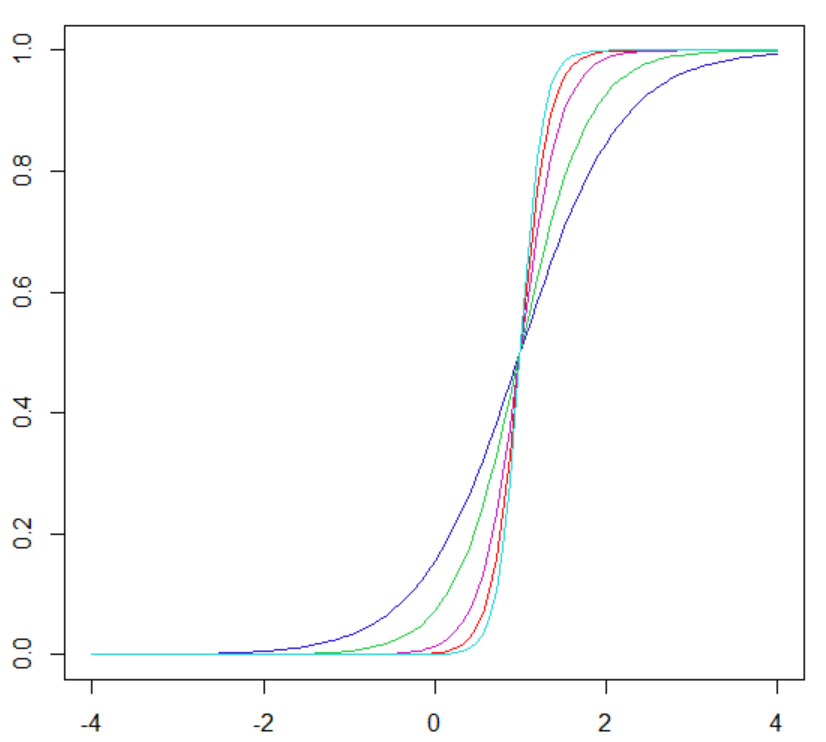
\includegraphics[bb = 650 470 1 1,scale = 0.25]{A.png}
    \vspace{4cm}
    \caption{$b$は$1$で固定、$a$は$-4, -2, 0, 2, 4$}
  \end{figure}
\end{frame}
\begin{frame}
  \begin{block}{$3$母数ロジスティックモデル}
  \begin{align}
    \displaystyle
    p_j(\theta) = c_j + \frac{1-c_j}{1+\exp(-Da_j(\theta - b_j))}
  \end{align}
  \begin{itemize}
    \item $2$母数ロジスティックモデルに加えて、偶然率$c_j$が追加されたモデル
    \item 下方漸近線といわれる
    \item 項目特性関数の各項目の正答率は$c_j$から$1$の間で推移する。
    \item $c$の値が大きくなるほど、グラフの下限が上がっていく。
  \end{itemize}
\end{block}
\end{frame}
\begin{frame}
  \begin{figure}[H]
    \centering
    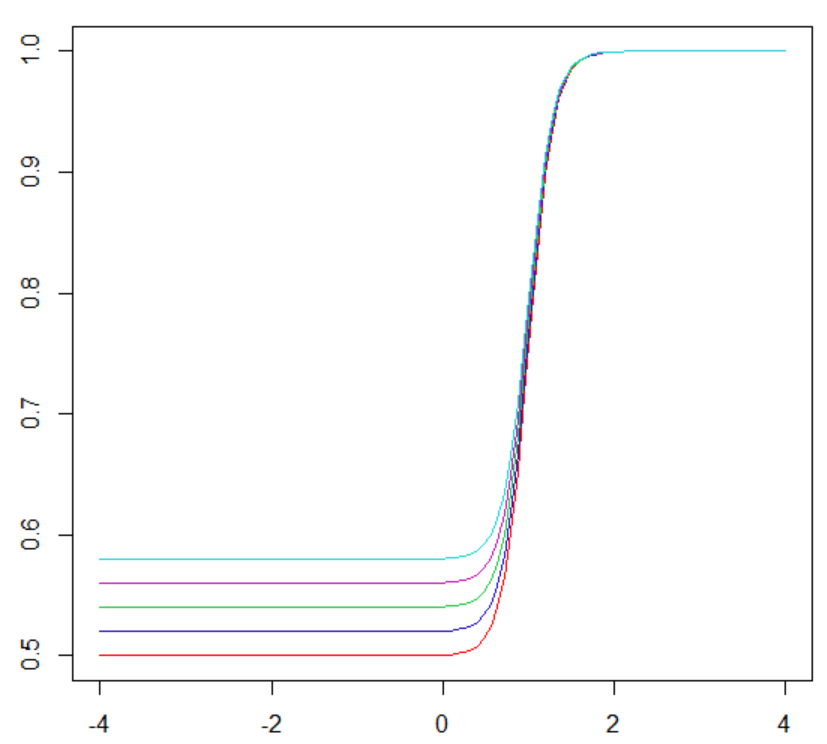
\includegraphics[bb = 650 470 1 1,scale = 0.25]{C.png}
    \vspace{4cm}
    \caption{$a$は$4$で固定、$b$は$1$で固定、$c$は$0.58, 0.56, 0.54, 0.52. 0.5$}
  \end{figure}
\end{frame}


\section{能力値や項目パラメータの推定}
\subsection{最尤推定法}
\begin{frame}
  \begin{block}{最尤推定法}
    項目パラメータが既知の場合に、項目パラメータと反応行列から能力値$\theta$の推定値を求める方法を紹介する。

  受験者$i$の能力値$\theta_i$は現実においては未知である。
  一方で、反応行列は収集して実際の値として固定し用いることができる。そこで、反応行列を既知として、能力値$\theta_i$を変数として扱うことにする。$L(\theta_i|\boldsymbol{u}_{i})$を次のように定義し、
  \begin{align}
    \label{01}
    \displaystyle L(\theta_i|\boldsymbol{u}_{i}) =\prod_{j = 1}^{n} p_{j}(\theta_i)^{u_{ij}} (1 - p_{j}(\theta_i))^{1 - u_{ij}}
  \end{align}
  この$L(\theta_i|\boldsymbol{u}_{i})$を尤度関数という。
  このとき、尤度が最大になるときの項目パラメータの値を、パラメータの推定値として利用する。このような推定法を最尤推定法という。つまり、この推定法は実際のデータが最も得られやすいようなパラメータの値を決める方法である。
  \end{block}
\end{frame}
\subsection{ベイズ推定法}
\subsubsection{EAP法(Expected a posteriori法)}
\begin{frame}
  \begin{block}{EAP法(Expected a posteriori法)}
    これは、$\theta_i$の事後分布の密度関数の$\theta_i$に関する平均値を推定値とする推定法である。これは、事後分布の平均が2乗損失を最小にするという事実に基づいた推定法である。式にすると、
    \begin{align}
      \displaystyle
      E[\theta_i | \boldsymbol{u}_i] = \int_{-\infty}^{+\infty} \theta_i \frac{p(\boldsymbol{u}_i | \theta_i)\pi(\theta_i)}{\displaystyle \int_{-\infty}^{+\infty} p(\boldsymbol{u}_i | \theta_i)\pi(\theta_i) d\theta_i} d\theta_i =  \frac{\displaystyle\int_{-\infty}^{+\infty} \theta_i \pi(\theta_i)p(\boldsymbol{u}_i|\theta) d\theta_i}{\displaystyle\int_{-\infty}^{+\infty}  \pi(\theta_i)p(\boldsymbol{u}_i|\theta) d\theta_i}
    \end{align}
    となる。ただし、$\pi(\theta)$は$\theta$の事前分布の密度関数である。式中の積分は区分求積法によって求めることができる。
  \end{block}
\end{frame}

\begin{frame}
  \begin{block}{EAP法(Expected a posteriori法)}
    能力値$\theta$だけでなく、項目パラメータに用いることで推定値を求めることができる。
    そのためには、項目パラメータの事前分布を仮定しておく必要がある。
    \begin{description}[labelwidth=10em]
      \item[能力値$\theta$の事前分布] 能力値$\theta$の事前分布には正規分布が仮定されることが多い。正規分布のパラメータは平均$\mu_\theta$と分散${\sigma}^2 _\theta$である。
      \item[識別力$a$の事前分布] 識別力の推定値は数学的には負の値もとり得るが、識別力の事前分布には正の範囲で定義される対数正規分布が仮定されることが多い。
      \item[困難度$b$の事前分布] 困難度の事前分布にも正規分布が仮定されることが多い。
      \item[偶然率$c$の事前分布] 偶然率の推定値は確率を表現するパラメータである。このため事前分布はベータ分布が仮定されることが多い。ベータ分布のパラメータは$\alpha,\beta$であり、密度関数は
      \begin{align}
        \displaystyle
        \frac{x^{\alpha - 1} (1 - x)^{\beta - 1}\Gamma(\alpha + \beta)}{\Gamma(\alpha) \Gamma(\beta)}
      \end{align}
      ベータ分布の最頻値は、
      \begin{align}
        \displaystyle
        \frac{\alpha - 1}{\alpha + \beta- 2}
      \end{align}
      であることが知られている。選択形式の問題の場合、偶然率の尤もらしい目安は選択肢数$k$の逆数$\frac{1}{k}$と考えられる。目安$\frac{1}{k}$を事前分布の最頻値の一致させるならば、例えば、
      \begin{align}
        \displaystyle
        \alpha = 20 \times \frac{1}{k} + 1\\
        \beta = 20 \times (1 - \frac{1}{k}) + 1
      \end{align}
      とする。$5$肢選択ならば$c = 0.2$とし$\alpha = 5,\beta = 17$のベータ分布を考える。
    \end{description}
  \end{block}
\end{frame}

\section{実際の推定}
\begin{frame}
  \begin{block}{実際の推定}
    \begin{itemize}
      \item $30$人の教育部学生に対して教育教養の問題を$8$問出題する。
    \end{itemize}
  \end{block}
  \begin{block}{反応行列}
    集計して反応行列$U$は以下のようになった。
        \[ \boldsymbol{U} =
    \left(
    \renewcommand{\arraycolsep}{3pt}
    \begin{array}{cccccccccccccccccccccccccccccc}
    1 & 0 & 0 & 0 & 1 & 0 & 0 & 1 & 0 & 1 & 0 & 0 & 0 & 0 & 0 & 0 & 0 & 1 & 0 & 0 & 0 & 0 & 1 & 0 & 1 & 1 & 0 & 0 & 1 & 1\\
    0 & 0 & 0 & 0 & 1 & 0 & 0 & 1 & 0 & 0 & 0 & 0 & 0 & 0 & 0 & 0 & 0 & 0 & 1 & 1 & 0 & 0 & 0 & 0 & 0 & 0 & 1 & 0 & 0 & 0\\
    0 & 0 & 0 & 1 & 0 & 0 & 0 & 0 & 1 & 0 & 0 & 0 & 0 & 0 & 1 & 0 & 0 & 0 & 0 & 0 & 1 & 1 & 1 & 0 & 0 & 0 & 0 & 0 & 0 & 0\\
    1 & 0 & 1 & 0 & 0 & 0 & 0 & 1 & 1 & 0 & 0 & 0 & 0 & 0 & 0 & 0 & 1 & 0 & 0 & 0 & 0 & 0 & 0 & 0 & 0 & 0 & 0 & 0 & 0 & 0\\
    0 & 0 & 1 & 0 & 0 & 1 & 1 & 0 & 0 & 0 & 1 & 0 & 0 & 0 & 1 & 0 & 0 & 0 & 1 & 0 & 0 & 0 & 0 & 0 & 0 & 0 & 1 & 0 & 0 & 0\\
    0 & 0 & 0 & 1 & 0 & 0 & 1 & 0 & 0 & 0 & 0 & 0 & 1 & 0 & 0 & 0 & 1 & 0 & 0 & 0 & 1 & 0 & 0 & 0 & 0 & 0 & 0 & 0 & 1 & 0\\
    1 & 0 & 0 & 0 & 1 & 0 & 0 & 1 & 1 & 0 & 0 & 0 & 1 & 0 & 0 & 0 & 1 & 1 & 0 & 0 & 1 & 0 & 1 & 0 & 1 & 1 & 0 & 0 & 1 & 0\\
    0 & 0 & 1 & 0 & 0 & 0 & 1 & 0 & 0 & 0 & 1 & 0 & 0 & 0 & 1 & 0 & 0 & 1 & 1 & 0 & 0 & 0 & 1 & 0 & 1 & 1 & 1 & 0 & 0 &0
    \end{array}
    \right)^t
    \]
  \end{block}
\end{frame}
\begin{frame}
  \begin{block}{実際の推定}
    $2$パラメータロジスティックモデルと$3$パラメータロジスティックモデルを用いて推定する。それぞれのパラメータの推定値は以下のようになった。
    \begin{table}[H]
      \begin{minipage}[t]{.45\textwidth}
        \begin{center}
          \begin{tabular}{|l||c|c|} \hline
            & 困難度& 識別力 \\ \hline \hline
            問題$1$ & $0.329$ & $0.369$  \\ \hline
            問題$2$ & $0.767$ & $0.843$  \\ \hline
            問題$3$ & $1.091$ & $0.705$   \\ \hline
            問題$4$ & $1.019$ & $0.766$   \\ \hline
            問題$5$ & $0.197$ & $3.083$   \\ \hline
            問題$6$ & $0.958$ & $0.534$   \\ \hline
            問題$7$ & $0.259$ & $0.431$   \\ \hline
            問題$8$ & $-0.18$ & $3.212$   \\ \hline
          \end{tabular}
        \end{center}
        \caption{$2$パラメータロジスティックモデル}
      \end{minipage}
      \begin{minipage}[t]{.45\textwidth}
        \vspace{-2.5cm}
        \begin{center}
          \begin{tabular}{|l||c|c|c|} \hline
            & 困難度& 識別力 & 偶然率\\ \hline \hline
            問題$1$ & $1.414$ & $1.622$ &$0.350$ \\ \hline
            問題$2$ & $0.958$ & $1.674$ &$0.140$ \\ \hline
            問題$3$ & $1.275$ & $1.787$ &$0.137$ \\ \hline
            問題$4$ & $1.274$ & $1.785$ &$0.136$ \\ \hline
            問題$5$ & $0.026$ & $2.970$ &$0.038$ \\ \hline
            問題$6$ & $1.334$ & $1.779$ &$0.200$ \\ \hline
            問題$7$ & $1.414$ & $1.623$ &$0.350$ \\ \hline
            問題$8$ & $-0.487$ & $3.175$ &$0.044$ \\ \hline
          \end{tabular}
        \end{center}
        \caption{$3$パラメータロジスティックモデル}
      \end{minipage}
    \end{table}
\end{block}
\end{frame}

\begin{frame}
  \begin{block}{考察}
    \vspace{4cm}
    \begin{figure}[H]
      \centering
      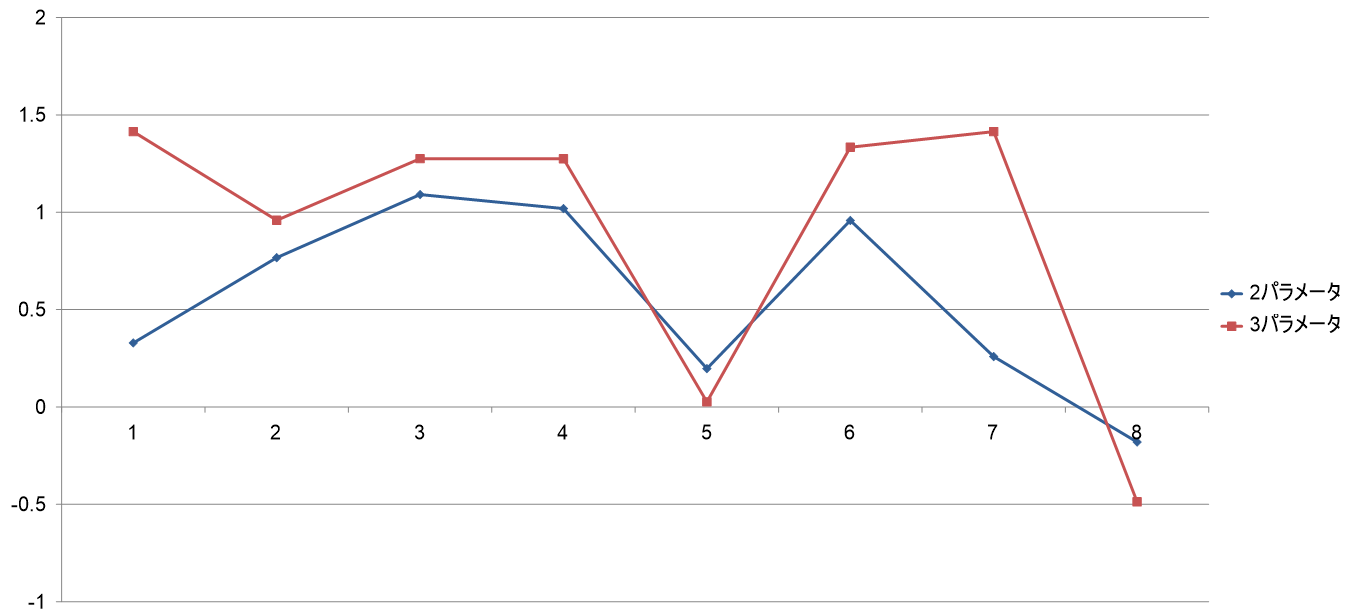
\includegraphics[bb = 1000 100 1 1,scale = 0.3]{maxmin.png}
      \vspace{1cm}
      \caption{困難度の推定値}
    \end{figure}
  \end{block}
\end{frame}

\begin{frame}
  \begin{block}{考察}
    \vspace{3.5cm}
    \begin{figure}[H]
      \centering
      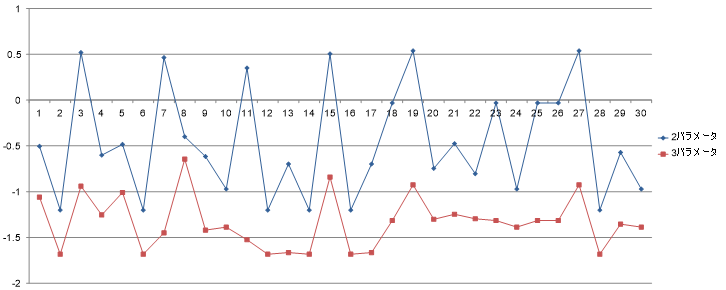
\includegraphics[bb = 550 100 1 1,scale = 0.7]{maxmin_theta.png}
      \vspace{2.5cm}
      \caption{能力値$\theta$の推定値}
    \end{figure}
  \end{block}
\end{frame}

\begin{frame}
  \begin{block}{考察}
    \vspace{3.5cm}
    \begin{figure}[H]
      \centering
      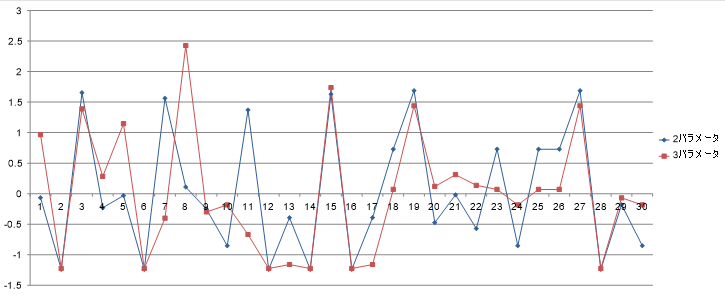
\includegraphics[bb = 550 100 1 1,scale = 0.7]{bay2bay3.png}
      \vspace{2.5cm}
      \caption{能力値$\theta$の推定値(標準化ver)}
    \end{figure}
  \end{block}
\end{frame}

\begin{frame}
  \begin{block}{最尤推定法との比較}
    最尤推定法も用いた推定値との比較もしていく。まずは、最尤推定法を用いた推定値とベイズ推定法の値($2$パラメータ)を表にまとめたものと能力値$\theta$を標準化しグラフに表したものを以下に示す。
    \begin{table}[H]
      \begin{minipage}[t]{.45\textwidth}
        \begin{center}
          \begin{tabular}{|l||c|c|} \hline
            & 困難度& 識別力 \\ \hline \hline
            問題$1$ & $0.329$ & $0.369$  \\ \hline
            問題$2$ & $0.767$ & $0.843$  \\ \hline
            問題$3$ & $1.091$ & $0.705$   \\ \hline
            問題$4$ & $1.019$ & $0.766$   \\ \hline
            問題$5$ & $0.197$ & $3.083$   \\ \hline
            問題$6$ & $0.958$ & $0.534$   \\ \hline
            問題$7$ & $0.259$ & $0.431$   \\ \hline
            問題$8$ & $-0.18$ & $3.212$   \\ \hline
          \end{tabular}
        \end{center}
        \caption{ベイズ推定法}
      \end{minipage}
      \begin{minipage}[t]{.45\textwidth}
        \vspace{-2.5cm}
        \begin{center}
          \begin{tabular}{|l||c|c|} \hline
            & 困難度& 識別力 \\ \hline \hline
            問題$1$ & $-6.87$ & $0.640$  \\ \hline
            問題$2$ & $-2.87$ & $0.841$  \\ \hline
            問題$3$ & $-0.87$ & $3.999$   \\ \hline
            問題$4$ & $0.461$ & $2.705$   \\ \hline
            問題$5$ & $1.461$ & $1.091$   \\ \hline
            問題$6$ & $2.261$ & $0.671$   \\ \hline
            問題$7$ & $2.928$ & $0.266$   \\ \hline
            問題$8$ & $3.499$ & $0.194$   \\ \hline
          \end{tabular}
        \end{center}
        \caption{最尤推定法}
      \end{minipage}
    \end{table}
  \end{block}
\end{frame}

\begin{frame}
  \begin{block}{考察}
    \vspace{4.5cm}
    \begin{figure}[H]
      \centering
      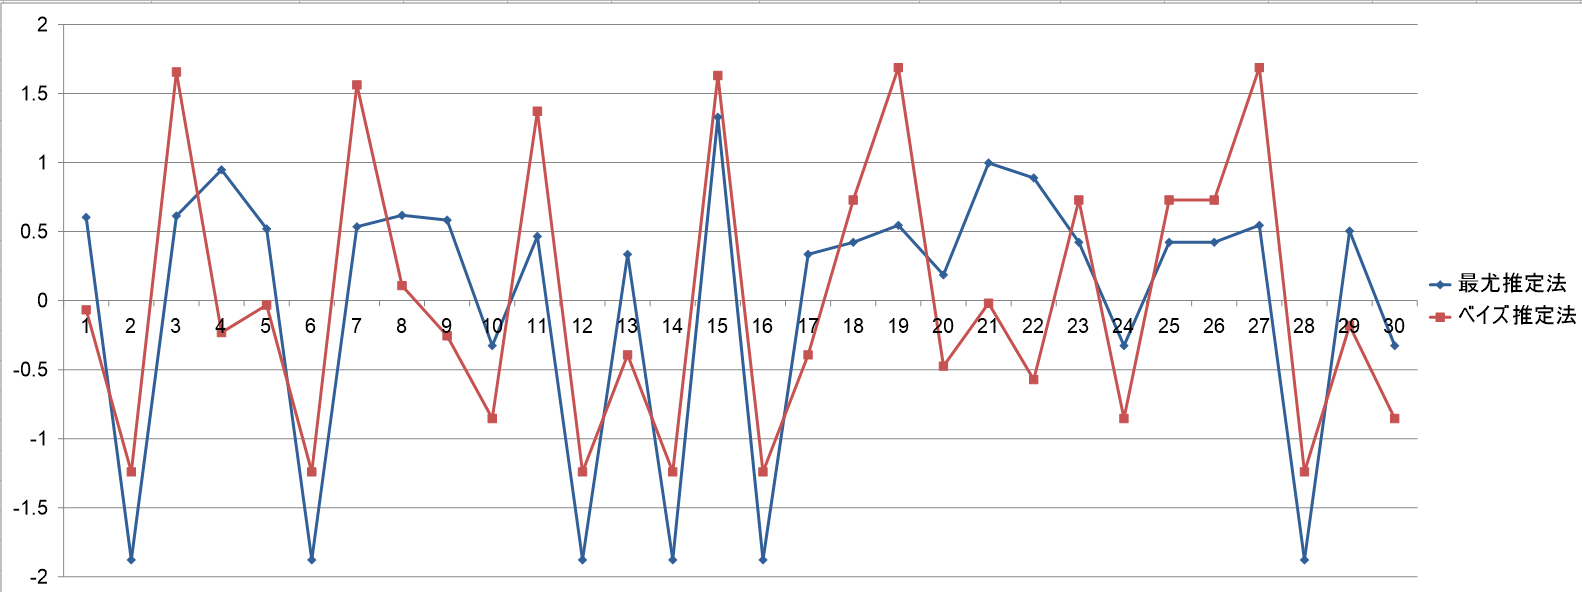
\includegraphics[bb = 1200 100 1 1,scale = 0.3]{saiyubay.png}
      \vspace{1cm}
      \caption{能力値$\theta$の推定値(標準化ver)}
    \end{figure}
  \end{block}
\end{frame}
\section{ロジスティックモデルの多次元化}
\subsection{多次元ロジスティックモデル}
\begin{frame}
  \begin{block}{多次元ロジスティックモデル}
    \begin{align}
      \displaystyle
      \label{4.1}
      p_j(\theta) = \frac{1}{1 + \exp(-\boldsymbol{{a}_j}^t \boldsymbol{\theta}_i + b_j)}
    \end{align}
    ここで$\boldsymbol{a}$は項目ごとの識別力を表すベクトルである。また、$\boldsymbol{\theta}$も受験者ごとの多次元の能力値を並べたベクトルである。つまり式中の$\boldsymbol{a}_j \boldsymbol{\theta_i} + b_j$は次のように表現することができる。
    \begin{align}
      \displaystyle
      \boldsymbol{{a}_j}^t \boldsymbol{\theta_i} + b_j = \sum_{l = 1}^{L} {a_{jl}}\theta_{il} + b_j
    \end{align}
    さらに、能力が$2$次元なものであるとし$\boldsymbol{\theta} = (\theta_1,\theta_2)^t$のように項目が受験者の違う$2$つ能力値を測定していると仮定する。
  \end{block}
\end{frame}

\begin{frame}
  \begin{block}{能力値や項目パラメータの推定}
    \begin{itemize}
      \item 識別力が高いものを選ぶべきなのか
      \item 困難度が高いものを選ぶべきなのか
      \item 過去問題は全体の中でどのくらいの割合で入れるべきなのか
    \end{itemize}
  \end{block}
\end{frame}
\subsection{シミュレーション}
\begin{frame}
  \begin{block}{計算の流れ}
    $100$人の受験者に$100$問の問題を解いてもらう。そのうち、一定の割合で項目パラメータが既知である問題を入れる。今回は過去問題が$25$問、$50$問、$75$問の$3$パターンで計算していく。計算の流れとしては、
\begin{itemize}
  \item[1] 過去問題と反応行列から新しい問題の項目パラメータを推定
  \item[2] 項目パラメータが推定された新しい問題を使って受験者の能力値を推定
\end{itemize}
の$2$段階に分ける。ここで以下の$2$点に注意されたい。
\begin{itemize}
  \item 過去問題のパラメータは既知扱いであるので、推定の対象外である。
  \item 受験者の能力値の推定には過去問題は使用せず、新しい問題だけを使用する。
\end{itemize}
  \end{block}
\end{frame}
\begin{frame}
  \begin{block}{パラメータの設定}
    \begin{itemize}
      \item $\boldsymbol{a_1} = (0.5, 0.53061, 0.56122, \cdots, 2, 0.5, 0.53061, 0.56122, \cdots, 2)$
      \item[]
      \item[]
      $\boldsymbol{a_2} = (0.5, 0.53061, 0.56122, \cdots, 1, 0.5, 0.53061, 0.56122, \cdots, 1)$
      \item $\boldsymbol{b} = (-1, -0.9797, -0.9595, \cdots, 1)$
      \item $\boldsymbol{\theta_1} = (-2, -1.9595, -1.9191, \cdots, 2)$
      \item[]
      \item[]
      $\boldsymbol{\theta_2} = (-1, -1, -1, \cdots, -1, 1, 1, \cdots, 1)$
    \end{itemize}
  \end{block}
\end{frame}

\begin{frame}
  \begin{block}{結果}
    以下に示すのは、能力値$\theta_1$、$\theta_2$の推定値と設定値との誤差の平均を、過去問題の割合毎にまとめたものである。
    \begin{table}[H]
      \begin{center}
        \begin{tabular}{|c||c|c|c|c|} \hline
          & 過去問題$0$問& 過去問題$25$問 & 過去問題$50$問 & 過去問題$75$問\\ \hline \hline
          $\theta_1$ & $0.397705342$	& $0.408443905$	& $0.416983791$	& $0.520276119$ \\ \hline
          $\theta_2$ & $0.488909176$	& $0.459919565$	& $0.5123526$	& $0.51364787$ \\ \hline
        \end{tabular}
      \end{center}
    \end{table}
  \end{block}
\end{frame}
\end{document}
